%% quantum's style

\documentclass[a4paper,twocolumn,11pt]{quantumarticle}

\pdfoutput=1
\usepackage[utf8]{inputenc}
\usepackage[english]{babel}
\usepackage[T1]{fontenc}
\usepackage{amsmath}
\usepackage{hyperref}
%
%\usepackage{tikz}
%\usepackage{lipsum}


%% our previous style and packages

%\documentclass[two column]{article}
%\usepackage[utf8]{inputenc}
\usepackage{graphicx}
\usepackage[dvipsnames]{xcolor}
%\usepackage[colorlinks=true,linkcolor=Blue,hypertexnames=false]{hyperref}
\usepackage{braket}
\usepackage{bbold}



\usepackage[numbers,sort&compress]{natbib}
%\usepackage[style=phys]{biblatex}
\usepackage{amssymb}
%\usepackage{amsmath}
\usepackage{placeins}
\usepackage{subcaption}

\usepackage[left=23mm,right=23mm,top=35mm,columnsep=15pt]{geometry}

\usepackage{pgfplotstable}
\usepackage{array}

\usepackage[qm]{qcircuit}

\usepackage{cancel}

\newcommand{\caro}[1]{\textcolor{red}{[#1]}}
\newcommand{\jovan}[1]{\textcolor{blue}{[#1]}}
\newcommand{\steve}[1]{\textcolor{purple}{[#1]}}




\title{Notes on $\mathbb{Z}_2$-SPT preparation protocols}
\author{Jovan Jovanovi\'c}
\affiliation{Rudolf Peierls Centre for Theoretical Physics, Parks Road, Oxford, OX1 3PU, UK}
\orcid{0000-0002-2508-3207}
\author{Carolin Wille}
\affiliation{Rudolf Peierls Centre for Theoretical Physics, Parks Road, Oxford, OX1 3PU, UK}
\orcid{0000-0002-9764-6937}
\author{Steven H. Simon}
\affiliation{Rudolf Peierls Centre for Theoretical Physics, Parks Road, Oxford, OX1 3PU, UK}
\orcid{0000-0001-7757-5978}



\date{11.08.2023.}

\begin{document}

\maketitle
\begin{abstract}
TBC  
\end{abstract}
\tableofcontents



\section{Overview}

Symmetry protected topological phases (SPTs) can be characterised by the properties of their fixed point wave-functions. Those properties are: \begin{enumerate}
\item Symmetric under an onsite representation of some symmetry group $G$.
\item It's parent Hamiltonian is gapped and it's ground state is unique, if the system lives on a closed manifold.
\item  If the manifold has an edge, a suitable parent Hamiltonian either supports a gapless edge mode or symmetry is spontaneously broken at the edge.
\end{enumerate}

Given the onsite symmetry group $G$ in $2+1$ dimensions we can classify all bosonic SPTs by the third cohomology group $\mathcal{H}^{3}(G, U(1))$ \cite{spt_coho_org}. Bosonic in this sense means that the elementary degrees of freedom commute, i.e. spin lattices. 

Given an element of the cohomology group $[\omega] \in \mathcal{H}^{3}(G, U(1))$ we can construct the fixed point wavefunction on a closed manifold.

For the case of concreteness we will immediately limit ourselves to the case at hand, $G = \mathbb{Z}_2$, its third cohomology group is $\mathcal{H}^{3}(\mathbb{Z}_2, U(1)) = \mathbb{Z}_2$. The two elements of the cohomology group represent the trivial paramagnet $\ket{\Psi_0}$ and our target state (the nontrivial SPT) $\ket{\Psi_1}$.

The two states are deceptively similar, given a spin-$1/2$ configuration on any lattice of $N$ sites the two states are: \begin{gather}
\ket{\Psi_0} = \sum_{\{s_i\}\in\{0,1\}^N}\ket{\{s_i\}}, \\ \ket{\Psi_1} = \sum_{\{s_i\}\in\{0,1\}^N}(-1)^{N_{d.w.}(\{s_i\})}\ket{\{s_i\}},
\end{gather} where $N_{d.w.}(\{s_i\})$ is the number of domain walls in a given configuration $\{s_i\}$. It is in the definition of this quantity that the embedding manifold plays a role.

\subsection{The fixed point Hamiltonian and Edge states}

Given a system made up of spin-$1/2$ occupying the sites of a regular triangular lattice we can construct a local Hamiltonian which is $\mathbb{Z}_2$-symmetric and whose ground state, $\ket{\Psi_1}$, is unique on a manifold without a boundary, \begin{equation}
H = - \sum_p h_p B_p.\label{eqn:ham}
\end{equation}
The sum in this expression goes over the sites $p$ and $h_p$ are any positive numbers (we will take to $h_p = 1$) since operators $B_p$ all commute. 
The operators $B_p$ themselves are defines as:\begin{equation}
B_p = \sigma^x_p \prod_{\langle pqq' \rangle} i^{\frac{1}{2}(1-\sigma^z_q\sigma^z_{q'})},
\end{equation}
where the sites in angled brackets mean that the three sites are a part of a triangle on a triangular lattice. See Figure \ref{fig:bp} for a schematic definition.\begin{figure}
\centering
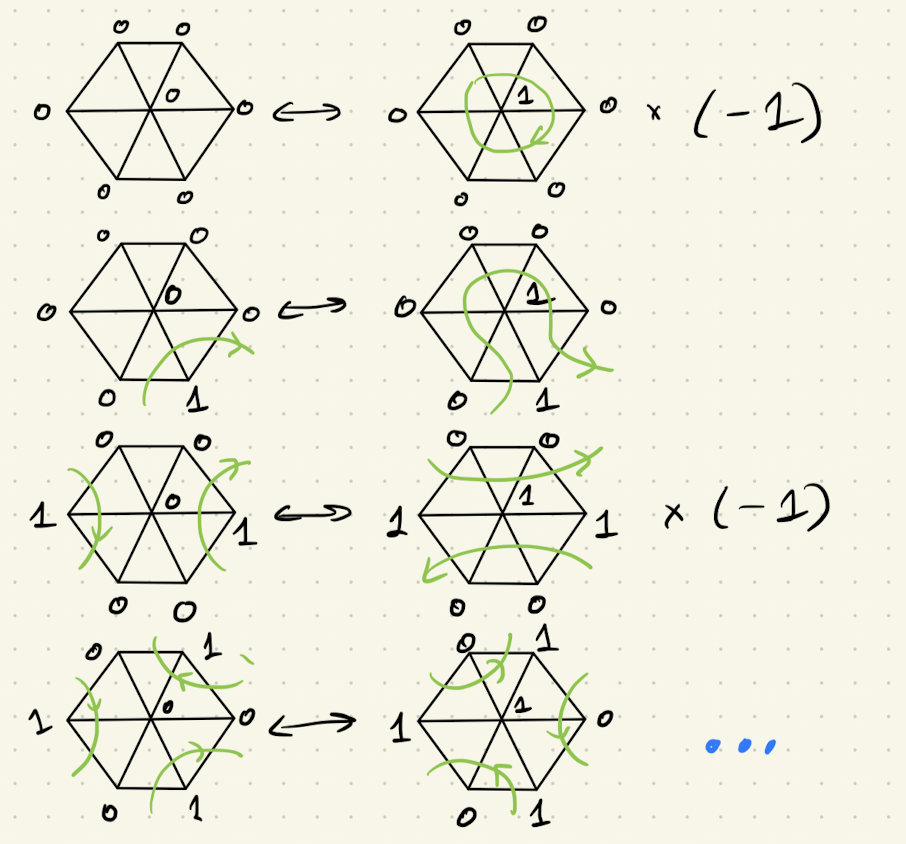
\includegraphics[width=\linewidth]{Figures/b_p.png}
\caption{The action of the operator $B_p$ on a site $p$ and triangles touching $p$, action is shown of a demonstrative set of basis vectors. The green lines represent the domain walls.}
\label{fig:bp}
\end{figure}
In essence, it flips a spin at a site $p$ and if that operation changes the domain wall parity (which can be determined locally) it add a $\pi$ phase shift, hence, it is clear that $\ket{\Psi_1}$ is fixed by all $B_p$-operators by definition.

This model was first proposed in 2012 by Levin and Gu \cite{levin-gu-z2}, for the reason of studying this phase of matter.

Once we open up a boundary we have left with a choice. We can divide up the sites into bulk sites $p \in R$ and boundary sites $\tilde p \in \partial R$, in the bulk the Hamiltonian is the same as for the manifold without boundary \begin{equation}
H = H_{\text{bulk}} + \cancelto{0}{H_{\text{edge}}} = \sum_{p \in R} B_p.\label{eqn:edge_bulk_ham}
\end{equation}
If we leave it at that we are left with a degenerate ground state manifold, the dimension of which is $|\mathcal{H}_{\text{edge}}| = 2^{|\partial R|}$ and whose basis can be chosen to be labelled by the boundary spin configuration.

As mentioned before the model is $\mathbb{Z}_2$ symmetric. On a manifold without boundary this symmetry is represented in a familiar on-site way $S = \prod_{p \in R} \sigma^x_p$. However, where this phase differentiates itself from the trivial para magnet is when an edge is involved.

If we choose, as mentioned, to label the states in the $\mathcal{H}_{\text{edge}}$ by the boundary spin configuration, $\ket{\{s_i\}_{\partial R}}$, we find \cite{levin-gu-z2} that the representation of the symmetry on this Hilbert space take this non on-site form \begin{equation}
S = - \prod_{i \in \partial R} \bar \sigma_i^x \exp{\left(\frac{i\pi}{4}\sum_{i \in \partial R}(1-\bar \sigma_i^z \bar \sigma_i^z)\right)}.
\end{equation}
We have to note that the Pauli operators in the above expression are not bare Pauli operators operating on the boundary physical spins, they also have an appropriate phase component depending on how the flip of the boundary spins affect the domain wall structure. In short, they act as Pauli operators but on the edge state labels themselves, $\{s_i\}_{\partial R}$. 

Given this symmetry action, we are free to explore possible edge extensions to our Hamiltonian. The fact that this symmetry action cannot stabilise a short-range entangled state (SRE, or an Matrix Product State) \cite{levin-gu-z2, Chen_2011} in the thermodynamic limit implies that any edge Hamiltonian cannot have it as a ground state. That is the reason behind the usual mantra, the edge of an SPT is either symmetry broken or gapless.

\subsection{Edge Physics}

\subsection{The String-Net Construction and F-moves}

Let us look at another way to define a fixed point wave-function of an SPT.
A wave-function of a $2+1$-dimensional SPO can be written as 
\section{State preparation}

We will introduce our lattice, see Figure \ref{fig:3x3pbc} for an example,
\begin{figure}
\centering
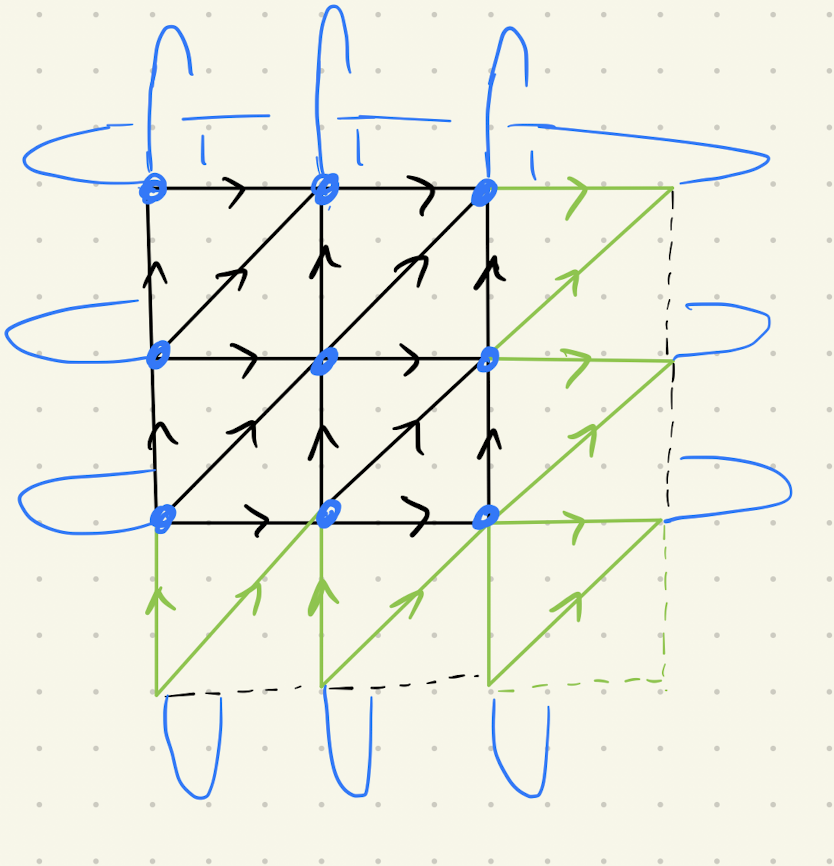
\includegraphics[width=\linewidth]{Figures/3x3_pbc.png}
\caption{An example of a N = 9 triangular lattice on a torus. (Proto)}
\label{fig:3x3pbc}
\end{figure}
in this example we have $N = 9$ spins on vertices of a triangular lattice on the periodic topology of a torus. For the sake of clarity we will drop the diagonal edges so we work with a simpler square lattice, only invoking the original stricture to resolve some ambiguities when it comes to defining $N_{d.w.}$ on a square lattice.

Given the simple structure of SPT states on closed manifolds, it is no surprise that there exist an efficient preparation protocol. In fact, once we prepare the trivial paramagnet we can just apply a phase to each plaquette according to a set of local plaquette rules, see Figure \ref{fig:plaq}.\begin{figure}
\centering
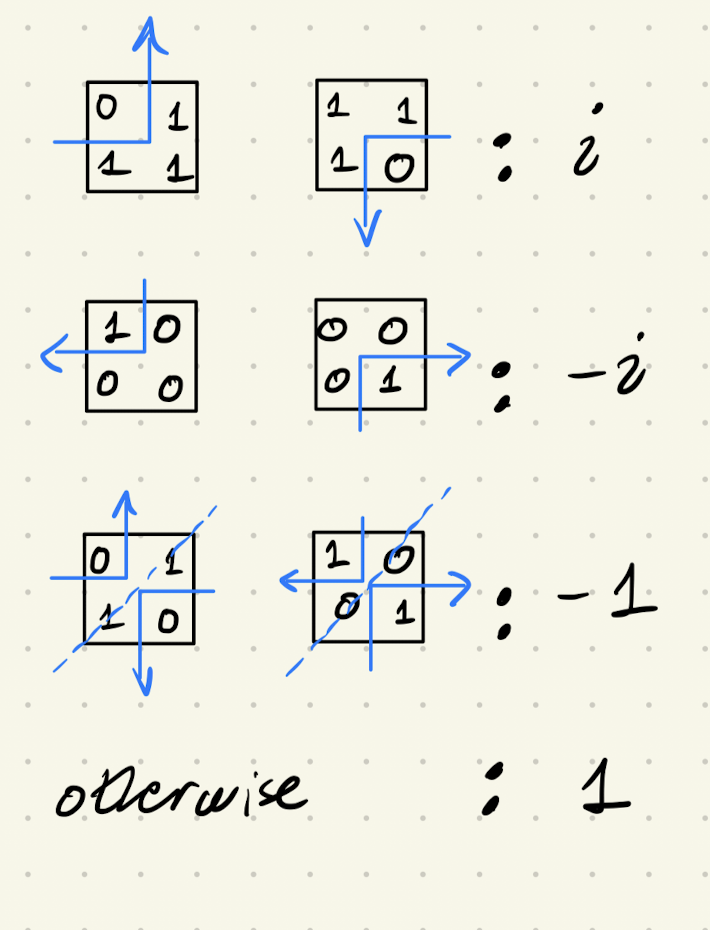
\includegraphics[width=\linewidth]{Figures/plaq_rules.png}
\caption{A set of plaquette rules that generate the correct phase factor on a closed manifold. (Proto)}
\label{fig:plaq}
\end{figure}
\begin{figure}
\centering
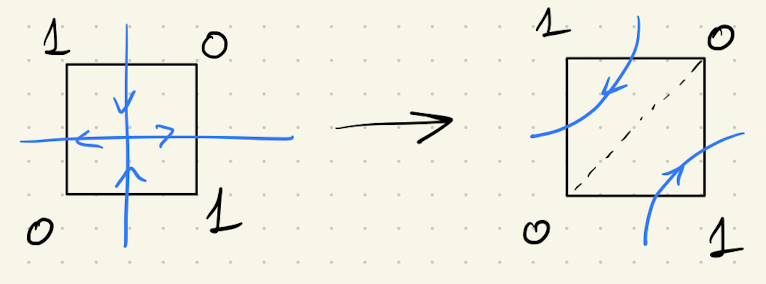
\includegraphics[width=\linewidth]{Figures/point_split.png}
\caption{The point splitting convention. The two ways of treating this edge case results in domain wall counts of opposite parity, to resolve this inconsistency we call on the original triangular lattice.}
\label{fig:point_split}
\end{figure}
To see this generates the correct phase, consider the case of one rectangular domain. It contributes with the phase $i \times i =  - 1$ ($-i \times -i =  - 1$) due to its two out of four corners contributing the adequate phase. Furthermore, introducing kinks and elongating the wall doesn't change the overall phase associated with that domain wall. Note that the rules are not compatible with the symmetries of the square precisely because the underlying structure is a triangular lattice.

It is also imperative to emphasise that these rules only reproduce the correct phase if we deal with a regular square lattice on a torus.
This, however, is far form the unique set of local rules. They are many that reproduce the same phase on a closed manifold, however thet all fail if the manifold has an edge (where domain walls enter and leave the system without closing).

\emph{Concrete protocol.} We will describe the concrete protocol for preparing a SPT fixed point wavefunction on a regular cubic lattice on a torus. 

Given the following layout of qubit's on the chip, see Figure \ref{fig:chip},
\begin{figure}
\centering
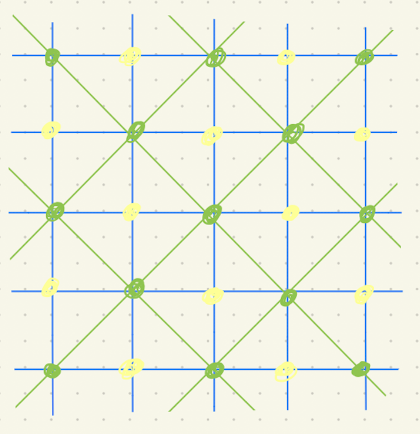
\includegraphics[width=\linewidth]{Figures/on_chip.png}
\caption{The layout of cubits on the chip. The green qubits represent the spin-1/2 physical degrees of freedom, while the yellow qubits (one per green plaquette) are used as auxiliary degrees of freedom. The blue links are representing the physical links between qubits on the chip over which we can implement two-qubit gates.}
\label{fig:chip}
\end{figure}
the protocol can be formulated in following six steps, see Figure \ref{fig:prot}.
\begin{figure}
\centering
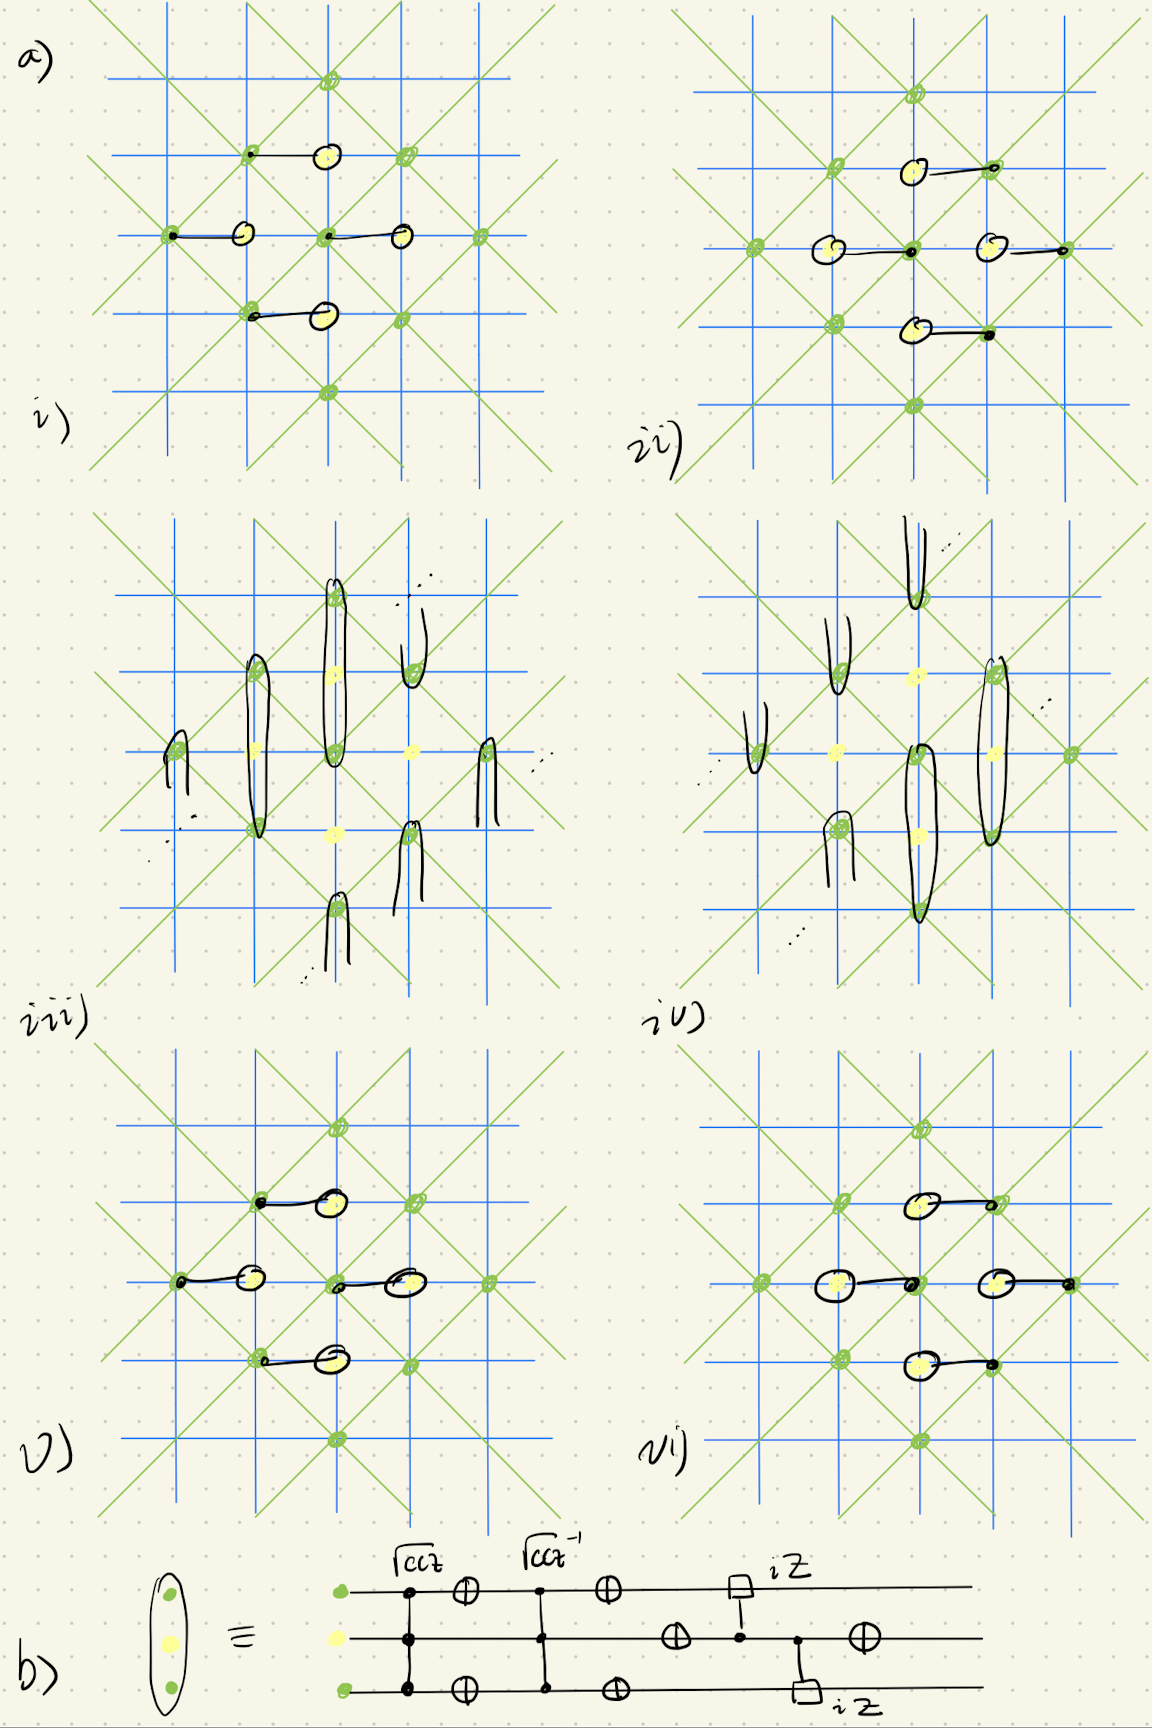
\includegraphics[width=\linewidth]{Figures/torus_protocol.png}
\caption{The six step protocol for preparing the $\mathbb{Z}_2$-SPT fixed point wavefunction on a regular square lattice on a torus.}
\label{fig:prot}
\end{figure}

The six steps are as follows:\begin{enumerate}
\item Given all states start in the state $\ket{0}$ apply a Haddamard gate to all green qubits (not shown in Figure \ref{fig:prot}),
\item Apply a CNOT gate from each green qubit to the auxiliary qubit to its left (Figure \ref{fig:prot}a.i.),
\item Apply a CNOT gate from each green qubit to the auxiliary qubit to its right (Figure \ref{fig:prot}a.ii.),
\item Apply the three-qubit circuit shown in Figure \ref{fig:prot}b. to the triples shown in Figure \ref{fig:prot}a.iii. implementing the local plaquette phase rules on the plaquettes in the odd rows,
\item Apply the three-qubit circuit shown in Figure \ref{fig:prot}b. to the triples shown in Figure \ref{fig:prot}a.iv. implementing the local plaquette phase rules on the plaquettes in the even rows,
\item Repeat steps 1. and 2. to disentangle the auxiliary qubits.
\end{enumerate}


\subsection{The Edge States and the "Bulk-Extension" circuit}

Let us examine what happens when there is an edge involved. 
Edge allows domain walls to enter and leave the system without closing.
Our protocol is designed to assign to each closed domain wall a phase of $e^{i\pi} = -1$ phase via the local plaquette phase rules which are predicated on the fact that closed domain walls will have a topologically invariant linear combination of left and right turns on a regular square lattice \begin{gather}
n_l  + n_r = \pm 4\\
n_l^{I} - n_r^{I} = \pm 2,\\
n_l^{II} - n_r^{II} = \pm 2.
\end{gather}
Last two equations come from the fact that also split the turn into two categories depending if they cross the main (present in the original triangular lattice picture) diagonal.  

For the domain walls that do not close we have do not have these invariants and our rules assign seemingly arbitrary phases, see Figure \ref{fig:edge_wall_phases}.
\begin{figure}
\centering
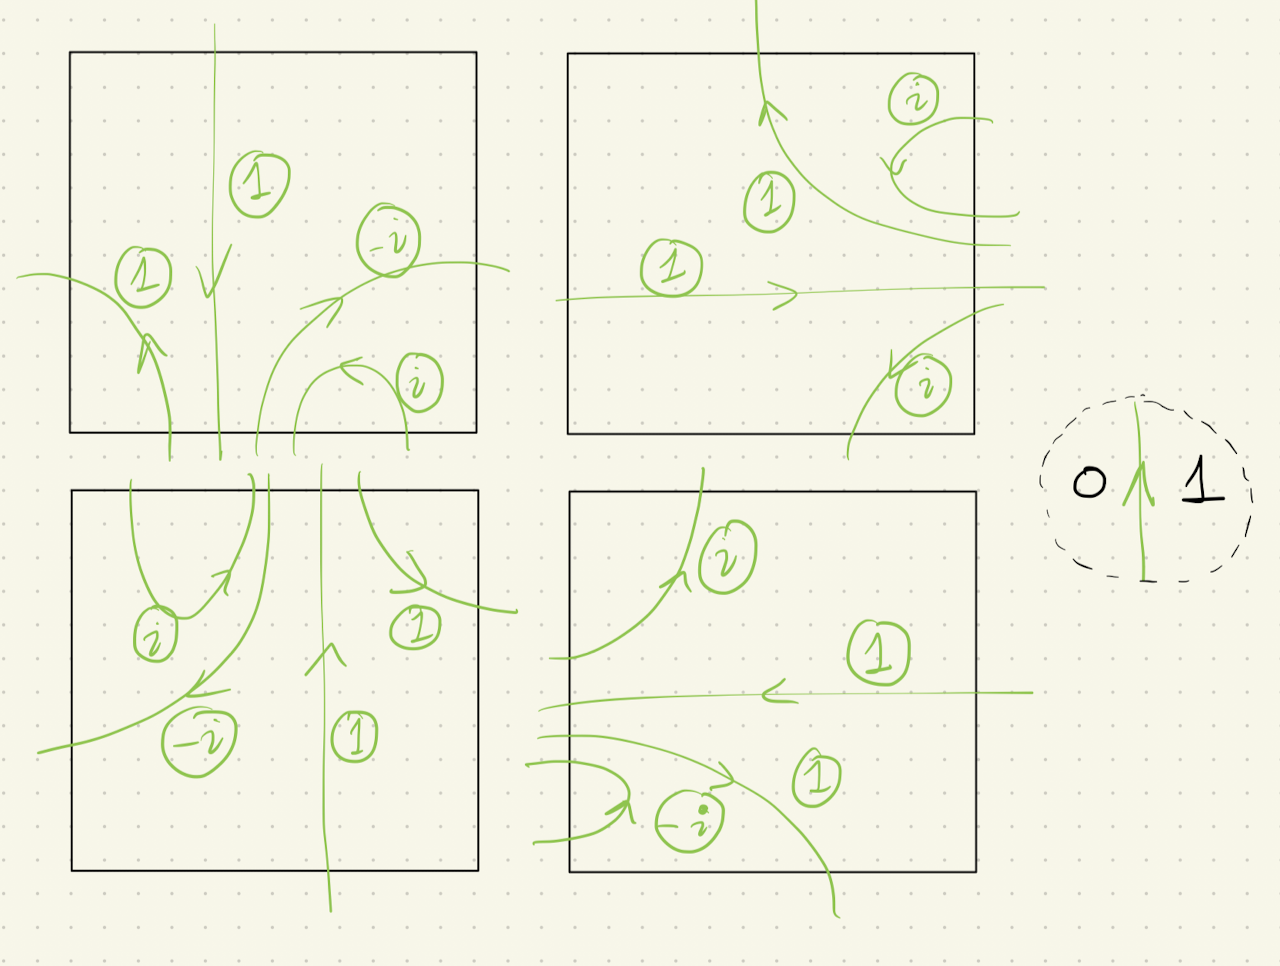
\includegraphics[width=\linewidth]{Figures/edge_wall_phases.png}
\caption{Deformation robust phases our algorithm assigns to domain walls entering and leaving the system via the edge.}
\label{fig:edge_wall_phases}
\end{figure}
For each edge spin configuration labelling our edge space $\mathcal{H}_{\text{edge}}$, the number of such domain walls is constant.
One would imagine that each of these walls needs to be associated with a phase of $-1$, however the resulting state would in fact not be stabilised by the Hamiltonian \eqref{eqn:edge_bulk_ham} in the bulk.

The phases associated with these walls must be compatible with the application of the F-moves in the bulk, which we checked that they are, se Figure \ref{fig:bulk_edge_move} for an example.\begin{figure}
\centering
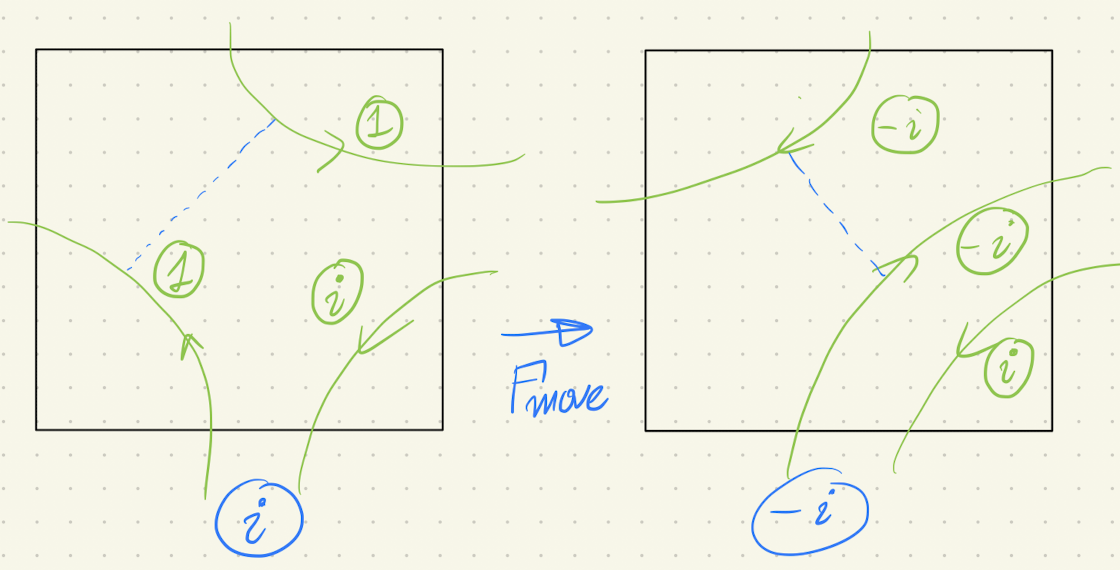
\includegraphics[width=\linewidth]{Figures/bulk_F_move.png}
\caption{An example of an F-move on the unclosed domain walls. The number of domain walls remains the same but the move will incur an additional $-1$ phase, covered by the phases assigned to the open domain walls by our algorithm.}
\label{fig:bulk_edge_move}
\end{figure}
Different protocols that reproduce the correct wave-function on a torus will have different phase assignments of these open domain walls, but will all be consistent with the bulk F-moves. This is due to the fact that the SPT edge basis states are short range entangled and the bulk plaquette terms $B_p$ will still be satisfied which implies consistency with bulk F-moves.

In general different protocols will just assign different phases to the edge basis states\begin{equation}
\ket{\{s_i\}_{\partial R}} \rightarrow e^{i\phi(\{s_i\}_{\partial R})}\ket{\{s_i\}_{\partial R}}.  
\end{equation}



%\printbibliography

\bibliographystyle{quantum}
\bibliography{bibliography}

\end{document}
